\chapter{المناعة الفطرية والالتهاب}\label{ch:b3:innate-immunity}

الشظية تحت الجلد تُدخل عشرة آلاف بكتيريا تتضاعف كل نصف
ساعة. وفي دقائق تتوسع الأوعية حولها وترشح؛ وفي ساعة تكون
أولى العدلات قد انسلّت من الدم وأخذت تزحف نحو الدخلاء على
أثر كيميائي؛ وفي يوم يصير الموضع أحمر حارًّا متورمًا موجعًا
--- وهي علامات \omterm{def:b3:innate-immunity:inflammation}{الالتهاب} الأربع التي عدّها كلسوس قبل ألفي
سنة --- وتكون البكتيريا قد ماتت، أكلتها حيةً خلايا عرفتها
غريبة من غير أن تكون قد لقيتها من قبل قط. تلك هي \omterm{def:b3:innate-immunity:innate}{المناعة
الفطرية}: الدفاع الذي لكل حيوان، الجاهز قبل الخمج، المكتوب
في الجينوم لا المتعلَّم. وهي سريعة، وهي التي تقتل معظم
الغزاة، وهي التي تخبر المناعة الأبطأ المتعلَّمة في الفصل
التالي أن هناك ما يُتعلَّم. وإفراطها --- الصدمة الإنتانية،
\omterm{def:b3:innate-immunity:inflammation}{والالتهاب} المزمن، وحمّيات الأمراض الالتهابية الذاتية ---
معلِّم كنجاحها.

\section{الطبقات والخلايا}

\begin{definition}[المناعة الفطرية]\label{def:b3:innate-immunity:innate}
\index{مناعة فطرية}\index{عدلة}\index{بلعمية}\index{خلية تغصنية}\index{خلية قاتلة طبيعية}\index{حاجز}
\emph{المناعة الفطرية} مجموعة الدفاعات الحاضرة قبل أي
تعرّض، المرمَّزة بمورّثات سلالة جرثومية لا تعيد ترتيب
نفسها، التي تتعرف سمات محفوظة في الميكروبات لا أفرادًا
بعينهم، وتعمل في دقائق إلى ساعات، وبلا ذاكرة (مع تحفظات).
وطبقتها الأولى هي \emph{الحواجز}: كيراتين الجلد، ومخاط
الطرق الهوائية وأهدابها، وحمض المعدة، وجَرف البول والدمع،
وإنزيم الليزوزيم الذي يقطع \omterm{def:b3:bacteriology:envelope}{الببتيدوغليكان}،
و\emph{الببتيدات الضدميكروبية} (الدفاعينات،
والكاثيليسيدينات) التي تثقب أغشية الميكروبات، \omterm{def:b3:microbiomes:symbiosis}{والميكروبيوم}
المعايش الذي يشغل الكُوى (\cref{ch:b3:microbiomes}).
وخلاياها كلها من السلالة النقوية إلا الأخيرة:
\emph{العدلات}، وهي \qty{60}{\%} من كريات الدم البيض، يُصنع
منها $10^{11}$ في اليوم وتعيش يومًا، وهي أول الواصلين وقاتلة
البكتيريا الكبرى؛ و\emph{البلعميات}، وهي مقيمات طويلات
العمر في كل نسيج (خلايا كوبفر في الكبد، والدبقيات الصغيرة
في الدماغ، والبلعميات السنخية في الرئة) تأكل وتنظف وتطلق
النذير؛ و\emph{الخلايا التغصنية}، التي تعاين النسج وتحمل ما
تجده إلى العقد اللمفية؛ والخلايا البدينة، والقاعدية،
والحمضية، مسلّحة ضد الطفيليات ومسؤولة عن الأرجية؛
و\emph{الخلايا القاتلة الطبيعية} (NK)، وهي لمفاويات تقتل
الخلايا المصابة أو المحوَّلة لأول نظرة.
\end{definition}

\begin{proof}[شواهد]
دفع ميتشنيكوف (1882)، في مسينة، شوكة وردة في يرقة نجم بحر
شفافة فرأى في صباح اليوم التالي خلايا متحركة تحتشد حولها؛
وكان قد رأى الخلايا نفسها تبتلع جسيمات الطعام وحبيبات
الصباغ، فافترض أنها تبتلع الميكروبات أيضًا --- وهي
\emph{البالعات}، عوامل دفاع مضيف تتبعه بعد ذلك في كل حيوان
قدر عليه، من الأميبات إلى الإنسان. وقد شارك إيرليش جائزة
نوبل لعام 1908، وكانت أضداده تمثّل الرأي الخلطي المقابل؛
وكان كلاهما مصيبًا، وبعد قرن تبيّن أن نصفي المناعة جهاز
واحد، وأن فطريّه يعلّم تكيّفيّه.
\end{proof}

\begin{omfigure}
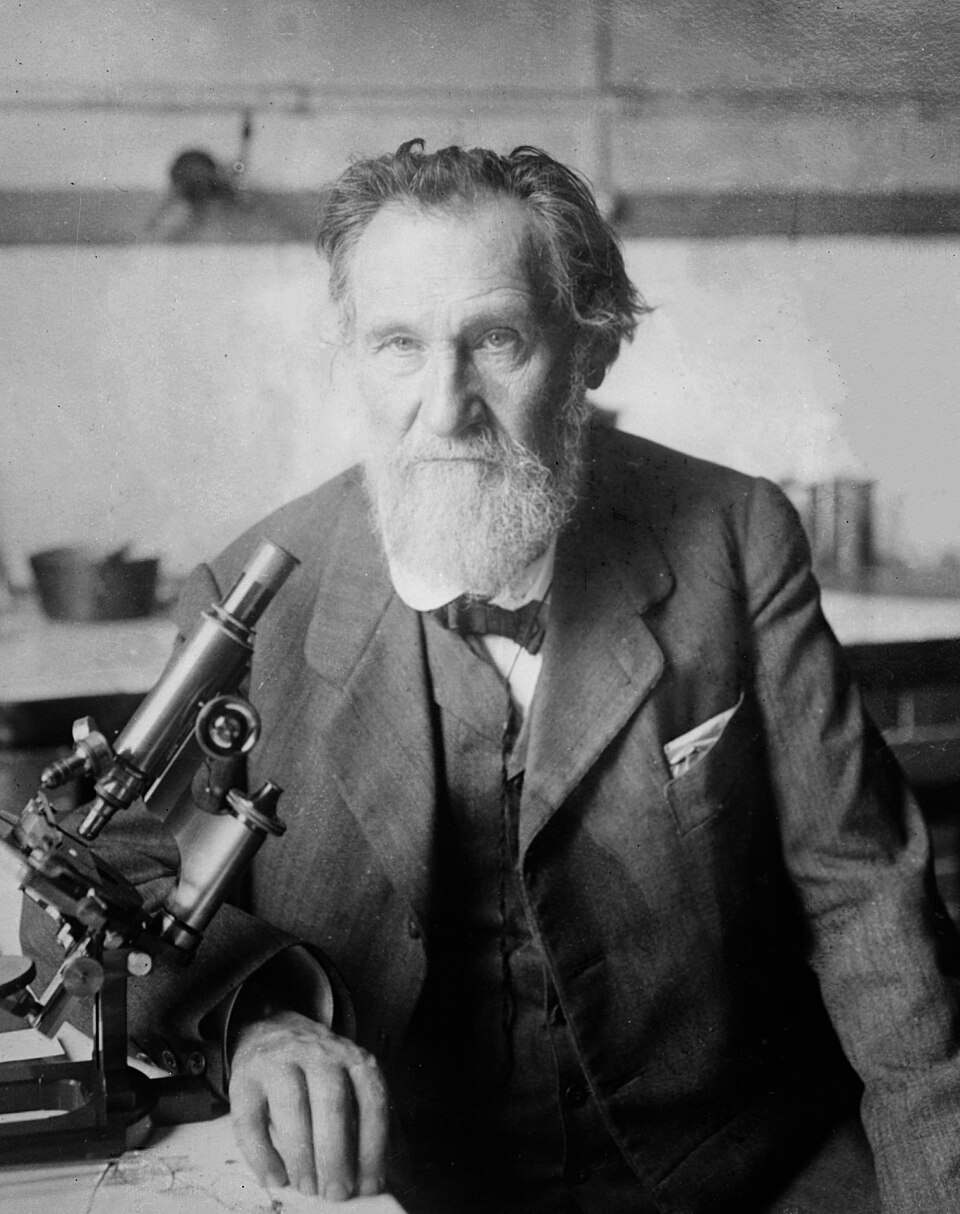
\includegraphics[width=0.30\linewidth]{images/book5/metchnikoff.jpg}\hspace{0.04\linewidth}
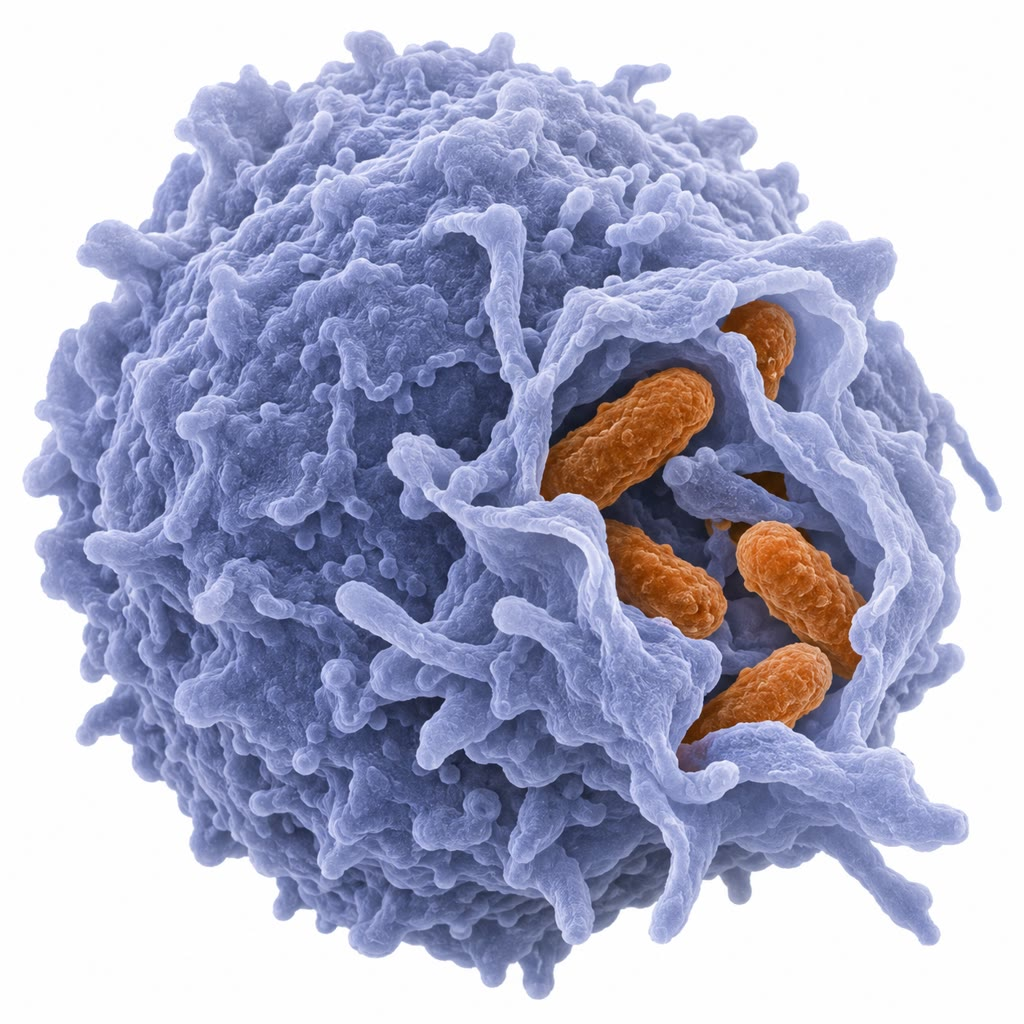
\includegraphics[width=0.30\linewidth]{images/book5/ai/b5-15-neutrophil-phagocytosis.jpg}\hspace{0.04\linewidth}
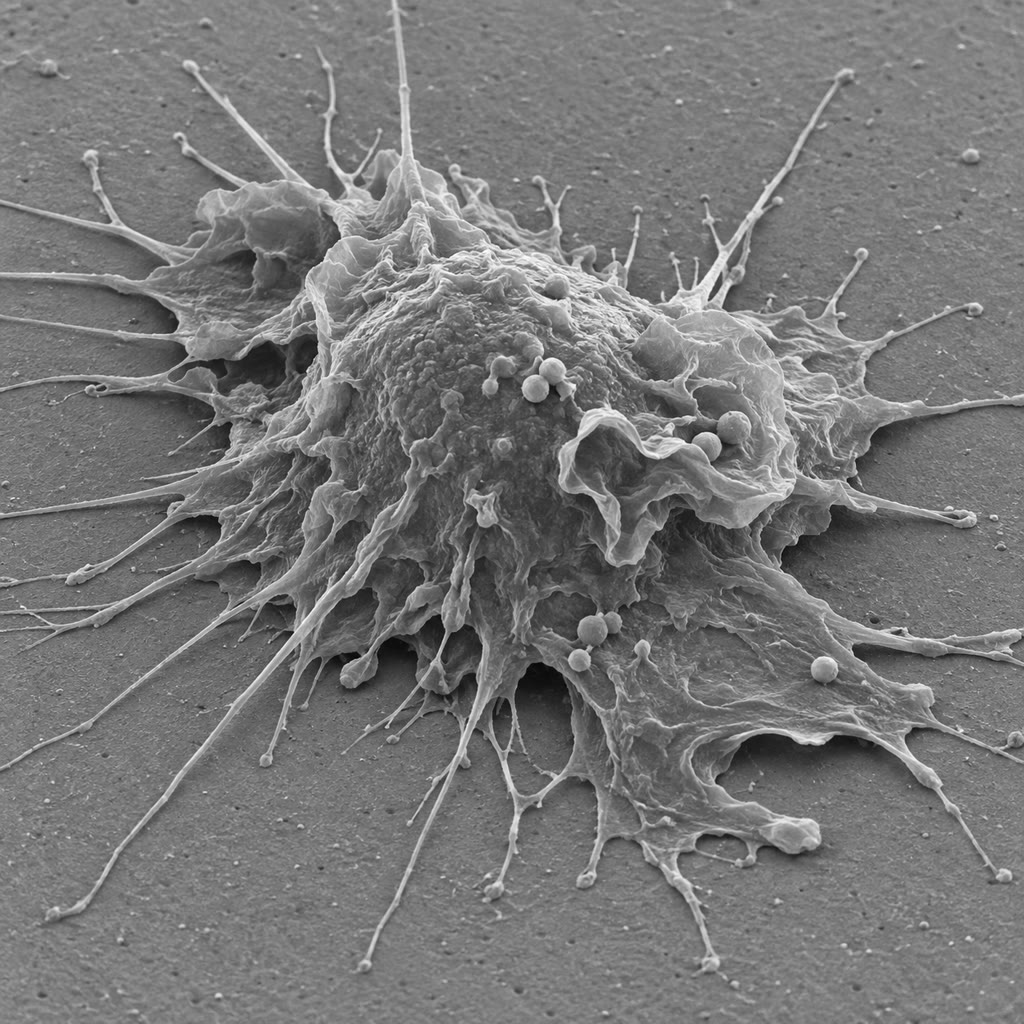
\includegraphics[width=0.30\linewidth]{images/book5/ai/b5-15-macrophage.jpg}

{\small إيلي ميتشنيكوف، الذي رأى البالعات تحتشد حول شوكة في
يرقة نجم بحر فأسس علم المناعة الخلوي (مكتبة الكونغرس، ملكية
عامة). وفي الوسط: \omterm{def:b3:innate-immunity:innate}{عدلة} تبتلع بكتيريا. ويمينًا: \omterm{def:b3:innate-immunity:innate}{بلعمية} تبسط
أغشيتها المكشكشة على سطح.}
\end{omfigure}

\section{التعرف على العدو}

\begin{definition}[التعرف على الأنماط]\label{def:b3:innate-immunity:prr}
\index{مستقبل تعرف الأنماط}\index{نمط جزيئي مرتبط بالممرضات}\index{مستقبل شبيه بمستقبل Toll}\index{نمط جزيئي مرتبط بالأذى}\index{جسيم التهابي}
تتعرف الخلايا الفطرية \emph{الأنماط الجزيئية المرتبطة
بالممرضات} (PAMP): وهي جزيئات مشتركة بين أصناف كاملة من
الميكروبات، ضرورية لها، وغائبة عن المضيف --- \omterm{def:b3:bacteriology:envelope}{عديد السكريد
الشحمي} في جدر سلبيات الغرام، \omterm{def:b3:bacteriology:envelope}{والببتيدوغليكان} وحمض التيكويك
الشحمي في إيجابياتها، والفلاجيلين، وغلوكانات $\beta$
الفطرية، وRNA مزدوج الطاق، وRNA بلا قلنسوة 5$'$، وDNA بثنائي
\omterm{def:b3:chromatin-epigenetics:methylation}{CpG} غير ممثيل، وDNA في العصارة الخلوية. والمستقبلات هي
\emph{مستقبلات تعرف الأنماط} (PRR)، وهي بضع عشرات في
مجموعها، كل منها مرمَّز بمورّثة واحدة: \emph{المستقبلات
الشبيهة بمستقبل Toll} (TLR) على السطح وفي الجسيمات الداخلية
(TLR4 \omterm{def:b3:bacteriology:envelope}{لعديد السكريد الشحمي}، وTLR5 للفلاجيلين، وTLR3 لجزيء
RNA مزدوج الطاق، وTLR9 لجزيء DNA ذي \omterm{def:b3:chromatin-epigenetics:methylation}{CpG})؛ وبروتينات NOD في
العصارة الخلوية لشظايا \omterm{def:b3:bacteriology:envelope}{الببتيدوغليكان}، وRIG-I لجزيء RNA
الفيروسي، وcGAS--STING لجزيء DNA في العصارة الخلوية؛
واللكتينات من النمط C لسكريات الفطور. وهذه المستقبلات
نفسها، أو غيرها من العائلات نفسها، تتعرف \emph{الأنماط
الجزيئية المرتبطة بالأذى} (DAMP) التي تطلقها الخلايا
المصابة بأذى --- ATP، وحمض البول، والبروتين النووي HMGB1،
وDNA المتقدرات --- فيلتهب الأذى العقيم أيضًا. ويفعّل
الارتباط عامل الاستنساخ NF-$\kappa$B والعوامل المنظِّمة
للإنترفيرون، فتشغّل السيتوكينات والكيموكينات وجزيئات
الالتصاق والمورّثات الضدميكروبية في غضون ساعة؛ وتجمّع طائفة
من المجسّات في العصارة الخلوية \emph{الجسيم الالتهابي}، وهو
منصة تفعّل الكاسباز-1 ليقطع الإنترلوكين-1$\beta$ إلى صورته
الفعالة وليطلق \omterm{def:b3:cell-cycle-apoptosis:other}{الموت الالتهابي} المسمى البيروبتوز
(\cref{ch:b3:cell-cycle-apoptosis}).
\end{definition}

\begin{proof}[شواهد]
اقترح جانواي عام 1989 أن الجهاز المناعي التكيّفي لا يستجيب
للمستضد وحده بل يحتاج إلى إشارة من مستقبلات فطرية تكون قد
تعرفت أنماطًا ميكروبية --- وهو تفسير حاجة اللقاحات إلى مواد
مساعدة، ``سرّ عالِم المناعة الصغير القذر''. ووجد هوفمان
(1996) أن \emph{Drosophila} التي تفتقر إلى المستقبل Toll،
المعروف بدوره في تنميط الجنين، لا تقدر على استنفار استجابة
ضد الفطور فتموت مغطاة بالعفن؛ وردّ بويتلر (1998) مقاومة
سلالة فئران \omterm{def:b3:bacteriology:envelope}{لعديد السكريد الشحمي}، وهي سلالة نجت من جرعات
ذيفان داخلي قاتلة لغيرها وأخفقت في تصفية أخماج سلبيات
الغرام، إلى طفرة في النظير الثديي TLR4. فكان مستقبل الذيفان
الداخلي، المطلوب منذ خمسين سنة، مستقبل Toll.
\end{proof}

\begin{omfigure}
\begin{tikzpicture}[every node/.style={font=\scriptsize}, >=stealth]
  % membrane
  \draw[very thick, omDef] (0,3.0) -- (11.5,3.0); \draw[very thick, omDef] (0,2.7) -- (11.5,2.7);
  \node[above] at (0.5,3.05) {الخارج}; \node[below] at (0.5,2.65) {العصارة الخلوية};
  % TLR4 with LPS
  \draw[thick, fill=omProp!35] (2.2,2.4) rectangle (2.6,3.9); \draw[thick, fill=omProp!35] (2.9,2.4) rectangle (3.3,3.9);
  \fill[omThm] (2.75,4.1) circle (0.14); \node[above] at (2.75,4.25) {LPS (نمط PAMP)};
  \node[right, align=left] at (3.4,3.5) {ثنائي TLR4\\مع MD2};
  % signalling
  \node[draw, thick, rounded corners, fill=omDef!20] (myd) at (2.75,1.7) {MyD88، وكينازات};
  \node[draw, thick, rounded corners, fill=omDef!20] (nfkb) at (2.75,0.6) {إطلاق NF-$\kappa$B};
  \node[draw, thick, rounded corners, fill=omMeth!25, align=center] (genes) at (2.75,-0.8) {TNF، وIL-1$\beta$، وIL-6، وIL-8؛\\جزيئات الالتصاق؛ iNOS};
  \draw[->, thick] (2.75,2.4) -- (myd); \draw[->, thick] (myd) -- (nfkb); \draw[->, thick] (nfkb) -- (genes);
  \node[right, font=\tiny] at (3.3,1.2) {في غضون ساعة};
  % cytosolic sensors
  \node[draw, thick, rounded corners, fill=omProp!25, align=center] (rig) at (6.9,1.9) {RIG-I: جزيء RNA فيروسي\\cGAS--STING: جزيء DNA في العصارة};
  \node[draw, thick, rounded corners, fill=omMeth!25] (ifn) at (6.9,-0.2) {إنترفيرون النمط I};
  \draw[->, thick] (rig) -- node[midway, right] {IRF3، وIRF7} (ifn);
  \node[draw, thick, rounded corners, fill=omThm!20, align=center] (nlrp) at (10.9,1.9) {الجسيم الالتهابي NLRP3:\\بلورات، وATP، ومسام};
  \node[draw, thick, rounded corners, fill=omMeth!25, align=center] (il1) at (10.9,-0.8) {الكاسباز-1: إطلاق IL-1$\beta$\\وموت التهابي};
  \draw[->, thick] (nlrp) -- (il1);
  \draw[->, thick, dashed] (genes.south) -- ++(0,-0.5) -| (il1.south) node[pos=0.25, below, font=\tiny] {طليعة IL-1$\beta$ يوفرها سبيل TLR};
\end{tikzpicture}

{\small ثلاثة أذرع للتعرف على الأنماط. مستقبل سطحي شبيه
بمستقبل Toll يرتبط به \omterm{def:b3:bacteriology:envelope}{عديد السكريد الشحمي} فيشير عبر
NF-$\kappa$B إلى السيتوكينات الالتهابية؛ ومجسّات الحمض
النووي الفيروسي في العصارة الخلوية تستحث الإنترفيرون؛
\omterm{def:b3:innate-immunity:prr}{والجسيم الالتهابي} يحوّل الطليعة المخزونة للإنترلوكين-1 إلى
\omterm{def:b3:innate-immunity:inflammation}{السيتوكين} الفعال.}
\end{omfigure}

\begin{definition}[المتمّمة]\label{def:b3:innate-immunity:complement}
\index{متمّمة}\index{محوّلة C3}\index{أوبسنة}\index{مركّب مهاجمة الغشاء}\index{ذيفان تأقي}
\emph{المتمّمة} جهاز من نحو ثلاثين بروتينًا بلازميًا،
\qty{10}{\%} من غلوبولينات المصل، يَسِم الميكروبات ويهدمها
بشلال من التفعيلات الحالّة للبروتين. وتلتقي ثلاثة سُبل عند
شطر البروتين المركزي C3: السبيل \emph{التقليدي}، الذي يبدؤه
ارتباط C1q بأضداد على سطح (أو \omterm{prop:b3:innate-immunity:systemic}{بالبروتين المتفاعل C}، أو
بخلايا مستميتة)؛ والسبيل \emph{اللكتيني}، الذي يبدؤه
اللكتين الرابط للمانوز متعرفًا سكريات ميكروبية؛ والسبيل
\emph{البديل}، الذي يتحلمه فيه C3 عفويًا بمعدل منخفض فيلتصق
C3b الناتج بأي سطح يلقاه. ويبني كل سبيل \emph{محوّلة C3}،
وهي إنزيم يشطر مزيدًا من C3؛ ويبني C3b الذي تودعه تساهميًا
على السطح مزيدًا من المحوّلة بدوره --- في عروة تضخيم ---
حتى يُكسى الجرثوم بملايين من C3b في دقائق. وC3b
\emph{أوبسونين}: فالبالعات تحمل مستقبلات له وتأكل ما يكسوه.
والشظيتان الصغيرتان C3a وC5a \emph{ذيفانان تأقيان} يوسعان
الأوعية ويجذبان العدلات ويفعّلان الخلايا البدينة. وأما C5b
فيجمّع C6--C9 في \emph{مركّب مهاجمة الغشاء}، وهو مسام قطره
\qty{10}{nm} يحلّ سلبيات الغرام والفيروسات المغلَّفة. وتنجو
خلايا المضيف لأنها تحمل منظِّمات --- العامل H، وCD55، وCD59
--- تفكك المحوّلة وتسد المسام على أسطحها هي؛ وأما
الميكروبات، إذ تفتقر إليها، فتلتهمها العروة.
\end{definition}

\begin{theorem}[عروة المتمّمة مميِّزًا حركيًا]\label{thm:b3:innate-immunity:complement}
\index{متمّمة!عروة التضخيم}
ليكن $B(t)$ عدد جزيئات C3b المودعة على سطح. يُودع C3b بمعدل
ثابت صغير $k_{0}$ من الدوران الذاتي للبروتين
C3، ويبني كل C3b مودع محوّلةً تودع مزيدًا بمعدل
$a$ لكل C3b في الثانية، بينما تزيل المنظِّمات (في المضيف)
والانحلال فعالية المحوّلة بمعدل $d$ لكل C3b في الثانية:
\[
\frac{\mathrm{d}B}{\mathrm{d}t} = k_{0} + (a - d)\,B .
\]
وعلى سطح يكون فيه $a > d$ --- أي ميكروب بلا منظِّمات ---
ينمو $B(t) = \bigl[k_{0}/(a-d)\bigr]\bigl(e^{(a-d)t} - 1\bigr)$
نموًا أسيًا بثابت زمني $1/(a - d)$؛ وعلى سطح مضيف يكون فيه
$d > a$، يقترب $B$ من القيمة المستقرة الصغيرة $k_{0}/(d - a)$.
فالجزيئات نفسها، عند التراكيز نفسها، تودع مليون C3b على
جرثوم في دقائق قليلة وبضع عشرات على الخلية التي بجانبه:
فالتمييز بين الذات وغير الذات لا يصنعه التعرف بل تصنعه
إشارة $a - d$.
\end{theorem}
\begin{proof}
المعادلة خطية بمعاملات ثابتة. فعند $a \ne d$ تكون النقطة
الثابتة $B^{*} = -k_{0}/(a-d)$؛ وبكتابة $B = B^{*} + u$ يكون
$\mathrm{d}u/\mathrm{d}t = (a-d)u$، فيكون $u = u_{0}e^{(a-d)t}$، ومع
$B(0) = 0$ يكون $B(t) = \bigl[k_{0}/(a-d)\bigr](e^{(a-d)t} - 1)$. وعند $a > d$
ينمو ذلك بلا حد (حتى ينفد C3 أو ينفد السطح)؛ وعند $a < d$
يخمد الأسّي ويؤول $B \to k_{0}/(d-a) > 0$. وعند $k_{0} = 1$
في الثانية، و$a - d = \qty{0.1}{s^{-1}}$ على جرثوم، يكون $B(\qty{2}{min})
= 10(e^{12} - 1) \approx 1.6\times 10^{6}$؛ وعند $d - a =
\qty{0.1}{s^{-1}}$ على خلية مضيف يكون $B^{*} = 10$.
\end{proof}

\begin{omfigure}
\begin{tikzpicture}
\begin{axis}[
  width=0.66\linewidth, height=5.6cm,
  axis x line=bottom, axis y line=left,
  xmin=0, xmax=150, ymin=1, ymax=1e7, ymode=log,
  xlabel={ثوانٍ}, ylabel={C3b المودع},
  xlabel style={font=\small, at={(axis description cs:0.5,-0.12)}, anchor=north}, ylabel style={font=\small},
  tick label style={font=\small}, xtick={0,30,60,90,120,150},
  clip=false,
]
\addplot[very thick, omThm, domain=1:150, samples=80] {10*(exp(0.1*x)-1)};
\addplot[very thick, omDef, domain=1:150, samples=80] {10*(1-exp(-0.1*x))};
\node[font=\scriptsize, omThm, anchor=east] at (axis cs:100,2e5) {ميكروب: $a > d$، أسّي};
\node[font=\scriptsize, omDef, anchor=south west] at (axis cs:60,14) {خلية مضيف: $d > a$، تشبع عند $k_{0}/(d-a)$};
\end{axis}
\end{tikzpicture}

{\small عروة \omterm{def:b3:innate-immunity:complement}{المتمّمة} على سطحين عند $k_{0} = 1$ في الثانية
و$|a - d| = \qty{0.1}{s^{-1}}$: فعلى ميكروب يفتقر إلى
المنظِّمات ينمو C3b نموًا أسيًا ويبلغ مليونًا في دقيقتين؛
وعلى خلية مضيف ذات منظِّمات يستوي عند عشرة.}
\end{omfigure}

\begin{omfigure}
\begin{tikzpicture}[every node/.style={font=\scriptsize}, >=stealth]
  \node[draw, thick, rounded corners, fill=omDef!20, align=center] (cl) at (-4.2,3.0) {تقليدي:\\C1q على ضد\\أو على البروتين المتفاعل C};
  \node[draw, thick, rounded corners, fill=omDef!20, align=center] (le) at (0,3.0) {لكتيني:\\اللكتين الرابط للمانوز\\على سكريات ميكروبية};
  \node[draw, thick, rounded corners, fill=omDef!20, align=center] (al) at (4.2,3.0) {بديل:\\دوران C3 الذاتي العفوي،\\C3b على أي سطح};
  \node[draw, thick, rounded corners, fill=omProp!35, minimum width=3cm] (conv) at (0,1.2) {محوّلة C3};
  \node[draw, thick, rounded corners, fill=omThm!25, align=center] (c3b) at (0,-0.4) {C3 $\to$ C3b (على السطح) $+$ C3a};
  \draw[->, thick] (cl) -- (conv); \draw[->, thick] (le) -- (conv); \draw[->, thick] (al) -- (conv);
  \draw[->, thick] (conv) -- (c3b);
  \draw[->, very thick, omThm] (c3b.east) .. controls (3.2,-0.4) and (3.2,1.2) .. (conv.east) node[pos=0.5, right, align=left] {عروة التضخيم:\\C3b يبني مزيدًا من المحوّلة};
  \node[draw, thick, rounded corners, fill=omMeth!25, align=center] (ops) at (-4.4,-2.2) {أوبسنة:\\البالعات تأكل\\ما يكسوه C3b};
  \node[draw, thick, rounded corners, fill=omMeth!25, align=center] (ana) at (0,-2.2) {C3a، وC5a:\\توسع الأوعية، وتجنيد العدلات\\والخلايا البدينة};
  \node[draw, thick, rounded corners, fill=omMeth!25, align=center] (mac) at (4.4,-2.2) {C5b--C9:\\مركّب مهاجمة الغشاء،\\حلّ};
  \draw[->, thick] (c3b) -- (ops); \draw[->, thick] (c3b) -- (ana); \draw[->, thick] (c3b) -- (mac);
  \node[draw, thick, rounded corners, fill=gray!15, align=center] (reg) at (-4.4,1.2) {منظِّمات المضيف:\\العامل H، وCD55، وCD59};
  \draw[-|, thick, gray!60!black] (reg) -- (conv);
\end{tikzpicture}

{\small \omterm{def:b3:innate-immunity:complement}{المتمّمة}. ثلاثة طرق تبني \omterm{def:b3:innate-immunity:complement}{محوّلة C3}؛ ويبني C3b الذي
تودعه مزيدًا منها (عروة المبرهنة)، ويقوم C3b المودع
\omterm{def:b3:innate-immunity:complement}{بالأوبسنة}، وتُلهب الشظايا، ويحلّ المركّب الطرفي. وتحمل
خلايا المضيف منظِّمات تقطع العروة (وتسد المسام بجزيء CD59)
على أغشيتها هي.}
\end{omfigure}

\section{الالتهاب}

\begin{definition}[الالتهاب الحاد]\label{def:b3:innate-immunity:inflammation}
\index{التهاب}\index{سيتوكين}\index{كيموكين}\index{انسلال}\index{سيليكتين}\index{إنتغرين}
\emph{الالتهاب} استجابة النسيج المروَّى للأذى أو للخمج،
تنظّمها \emph{السيتوكينات} --- وهي بروتينات الإشارة الصغيرة
في الخلايا المناعية، وأهمها هنا TNF والإنترلوكين-1
والإنترلوكين-6 من البلعميات المفعَّلة ---
و\emph{الكيموكينات}، وهي السيتوكينات التي توجّه الهجرة.
وخطواته تفسر علامات كلسوس. فالهيستامين من الخلايا البدينة،
وأكسيد النتريك، والبروستاغلاندينات توسّع الشرينات: وذلك
\emph{الاحمرار} و\emph{الحرارة}. وتتقلص بطانة الوُرَيدات
فترشح البلازما، وتغمر بروتيناتُها --- \omterm{def:b3:innate-immunity:complement}{المتمّمة}، والأضداد،
وعوامل التخثر --- النسيجَ: وذلك \emph{التورم}. ويحسّس
البراديكينين والبروستاغلاندين E$_{2}$ النهايات العصبية:
وذلك \emph{الألم}. وتصل الكريات البيض عن طريق
\emph{الانسلال}: إذ يجعل TNF والإنترلوكين-1 البطانةَ تعرض
\emph{السيليكتينات}، التي تلتقط عليها العدلات المارّة
وتتدحرج؛ وتفعّل الكيموكينات (الإنترلوكين-8) على سطح البطانة
\emph{إنتغرينات} العدلات، فترتبط ارتباطًا وثيقًا بجزيئات
الالتصاق البطانية وتوقف الخلية؛ ثم تنسل \omterm{def:b3:innate-immunity:innate}{العدلة} بين خلايا
البطانة وتتبع تدرج الكيموكين إلى النسيج --- والمتوالية كلها
في دقائق قليلة، بما يبلغ مليون خلية في الساعة إلى موضع
مخموج.
\end{definition}

\begin{omfigure}
\begin{tikzpicture}[every node/.style={font=\scriptsize}, >=stealth]
  % vessel wall
  \fill[omThm!10] (0,0) rectangle (12,2.3); \node[left, omThm!70!black, anchor=north east] at (12,2.25) {الدم، جارٍ $\rightarrow$};
  \foreach \x in {0,1.5,3,4.5,6,7.5,9,10.5} \draw[thick, fill=omDef!30] (\x,-0.05) rectangle (\x+1.45,0.35);
  \node[right] at (0.1,-0.35) {البطانة};
  \fill[omMeth!8] (0,-1.7) rectangle (12,-0.45); \node[right, omMeth!60!black] at (0.1,-1.55) {النسيج};
  % bacteria and chemokine gradient
  \foreach \p in {(10.6,-1.1),(11.0,-0.9),(11.3,-1.2)} \fill[omProp] \p ellipse (0.14 and 0.07);
  \node[below, omProp] at (11.0,-1.35) {بكتيريا};
  \node[below, font=\tiny] at (8.0,-0.5) {تدرج الكيموكين $\rightarrow$};
  % neutrophils in sequence
  \draw[thick, fill=white] (1.2,1.1) circle (0.3); \node[above] at (1.2,1.45) {1. جريان};
  \draw[thick, fill=white] (3.4,0.68) circle (0.3); \node[above] at (3.4,1.05) {2. تدحرج على السيليكتينات};
  \draw[omThm, thick] (3.1,0.45) -- (3.05,0.35); \draw[omThm, thick] (3.4,0.38) -- (3.4,0.35); \draw[omThm, thick] (3.7,0.45) -- (3.75,0.35);
  \draw[thick, fill=white] (6.0,0.62) ellipse (0.38 and 0.26); \node[above, align=center] at (6.0,0.95) {3. التصاق وثيق\\(إنتغرينات)};
  \draw[thick, fill=white] (8.25,0.18) ellipse (0.2 and 0.42); \node[above, align=center] at (8.4,0.95) {4. انسلال\\عبر الجدار};
  \draw[thick, fill=white] (9.6,-1.0) circle (0.3); \node[left] at (9.25,-1.0) {5. زحف إلى الموضع};
  \draw[->, thick, gray] (1.5,1.05) -- (3.0,0.8); \draw[->, thick, gray] (3.7,0.68) -- (5.6,0.62); \draw[->, thick, gray] (6.4,0.5) -- (8.0,0.4); \draw[->, thick, gray] (8.3,-0.3) -- (9.3,-0.8);
  % TNF label
  \node[below, align=center, font=\tiny] at (4.0,-1.75) {TNF وIL-1 من بلعميات النسيج يجعلان البطانة\\تعرض السيليكتينات وجزيئات الالتصاق التي تلتقط العدلات};
\end{tikzpicture}

{\small \omterm{def:b3:innate-immunity:inflammation}{الانسلال}. سيتوكينات من بلعميات النسيج تجعل جدار
الوُرَيد لزجًا؛ فتلتقط \omterm{def:b3:innate-immunity:innate}{عدلة} مارّة على السيليكتينات
وتتدحرج، وتوقفها إنتغريناتها، فتنسل بين خلايا البطانة،
وتتبع تدرج \omterm{def:b3:innate-immunity:inflammation}{الكيموكين} إلى البكتيريا.}
\end{omfigure}

\begin{proposition}[الحمّى، والطور الحاد، والانحلال]\label{prop:b3:innate-immunity:systemic}
\index{حمّى}\index{استجابة الطور الحاد}\index{بروتين متفاعل C}\index{انحلال الالتهاب}
يعمل الإنترلوكين-1 وTNF والإنترلوكين-6 عن بُعد أيضًا. ففي
الوطاء تستحث البروستاغلاندين E$_{2}$، الذي يرفع نقطة ضبط
حرارة الجسم: وتلك \emph{الحمّى}، التي تبطئ كثيرًا من
البكتيريا، وتسرّع تفاعلات الخلايا المناعية نفسها، وتكلف نحو
\qty{12}{\%} استقلابًا إضافيًا لكل درجة. وفي الكبد تستحث
\emph{بروتينات الطور الحاد} --- \omterm{prop:b3:innate-immunity:systemic}{البروتين المتفاعل C}، الذي
يربط فسفوكولين البكتيريا ويفعّل \omterm{def:b3:innate-immunity:complement}{المتمّمة} ويرتفع ألف ضعف في
يومين، وهو مقياس الطبيب \omterm{def:b3:innate-immunity:inflammation}{للالتهاب}؛ والفيبرينوجين؛ واللكتين
الرابط للمانوز؛ والهيبسيدين، الذي يحبس الحديد عن الميكروبات
التي تحتاج إليه. وفي النقي تطلق العدلات وتسرّع إنتاجها.
\omterm{def:b3:innate-immunity:inflammation}{والالتهاب} مقدَّر له أن ينتهي: فمع تصفية المنبّه تتحول
الوسائط الشحمية من البروستاغلاندينات إلى الليبوكسينات
والريزولفينات، وتموت العدلات استماتةً فتأكلها البلعميات،
التي تنتقل عندئذ إلى برنامج إصلاح، فتفرز عوامل نمو
والإنترلوكين-10 --- وذلك \emph{الانحلال}. وحين يدوم المنبّه
(عصية سل لا تُقتل، أو بلورة، أو مستضد ذاتي) تصير الاستجابة
مزمنة: فتسوّر البلعميات الموضع في \omterm{def:b3:cancer-biology:hallmarks}{ورم} حبيبي، وتضع الأرومات
الليفية ندبة، ويُهدم النسيج بدفاعه هو.
\end{proposition}

\begin{example}[الإنتان]\label{ex:b3:innate-immunity:sepsis}
\omterm{def:b3:innate-immunity:inflammation}{الالتهاب} المحصور في شظية شفاء؛ وأما التفاعلات نفسها في
الجسم كله فكارثة. فحين تبلغ البكتيريا أو \omterm{def:b3:bacteriology:envelope}{عديد السكريد
الشحمي} الدمَ بكميات، تطلق البلعميات في كل مكان TNF
والإنترلوكين-1 دفعة واحدة: فيتوسع كل وعاء ويرشح، وينهار ضغط
الدم، ويُفعَّل التخثر في عشرة آلاف شعيرة فيستهلك عوامل
التخثر، وتخفق الأعضاء إذ تُحرم الإرواء --- وتلك
\emph{الصدمة الإنتانية}، التي تقتل ربع من تصيبهم إلى نصفهم،
أي نحو أحد عشر مليون إنسان في السنة. وبضعة ميكروغرامات من
\omterm{def:b3:bacteriology:envelope}{عديد السكريد الشحمي} تُحقن في متطوع تُحدث حمّى ونافضًا
وهبوطًا في ضغط الدم في غضون ساعتين؛ وفأر يفتقر إلى TLR4 لا
يبالي بجرعة تقتل غيره مئة مرة. فالمرض هو استجابة المضيف،
والصادات التي تقتل البكتيريا قد تزيده سوءًا ساعات قليلة
بإطلاق مزيد من الذيفان الداخلي.
\end{example}

\begin{omfigure}
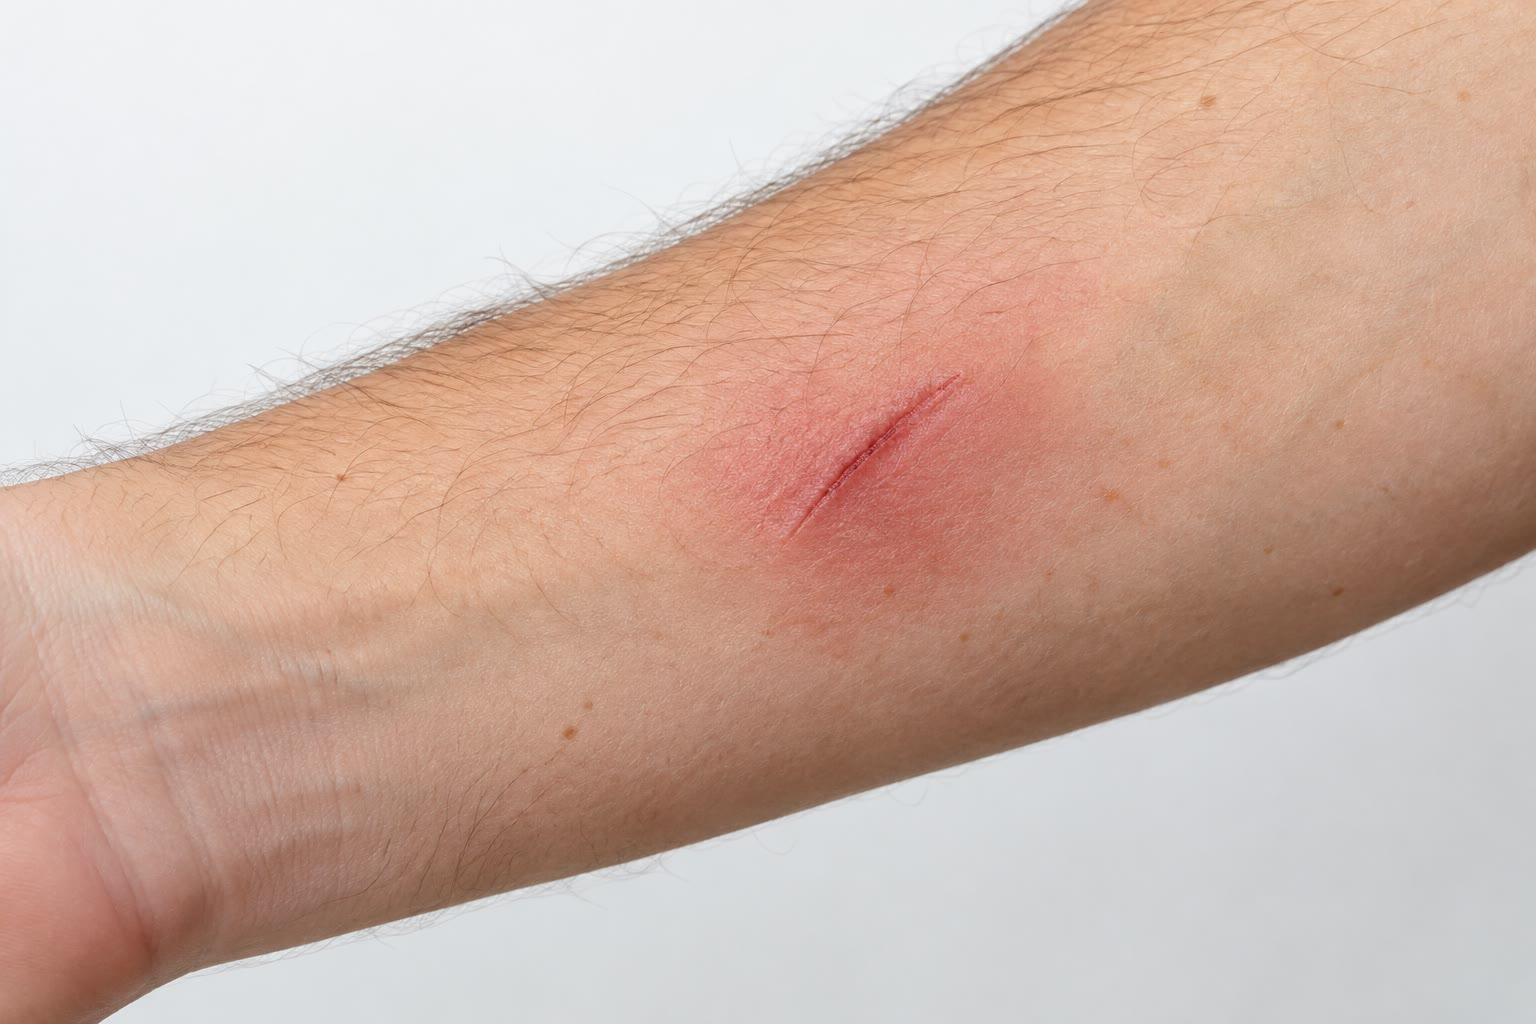
\includegraphics[width=0.52\linewidth]{images/book5/ai/b5-15-inflamed-skin.jpg}

{\small \omterm{def:b3:innate-immunity:inflammation}{التهاب} حاد حول خدش شوكة: احمرار ودفء من الأوعية
المتوسعة، وتورم من البلازما الراشحة، والألم الذي يبقي الطرف
ساكنًا --- وهي الاستجابة الموضعية التي تكون، إذا عُمّمت على
الجسم كله، صدمةً إنتانية.}
\end{omfigure}

\section{القتل}

\begin{definition}[البلعمة والانفجار التنفسي]\label{def:b3:innate-immunity:killing}
\index{بلعمة}\index{انفجار تنفسي}\index{أكسيداز NADPH}\index{شبكة العدلة خارج الخلوية}
تربط البالعة فريستها بمستقبلات للأوبسونينات --- C3b،
والمناطق الثابتة من الأضداد --- أو مباشرةً بمستقبلات
الأنماط، ثم تلفها في غشاء وتغلق \emph{الجسيم البلعمي}، الذي
يندمج مع الحبيبات والجسيمات الحالّة. والقتل بعدة وسائل
معًا. فأولها \emph{الانفجار التنفسي}: إذ يضخ إنزيم
\emph{أكسيداز NADPH}، المجمَّع على غشاء الجسيم البلعمي،
إلكترونات على الأكسجين ليصنع فوق الأكسيد، الذي يصير فوق
أكسيد الهدروجين، الذي تحوّله بيروكسيداز النقويات، مع
الكلوريد، إلى هيبوكلوريت --- أي مُبيّضًا، عند تركيز ميلي
مولاري داخل حجيرة عرضها ميكرومتر. ثم أكسيد النتريك من سنثاز
NO المستحث، الذي يعطي مع فوق الأكسيد فوق النتريت. والحمض،
إلى pH~5. والليزوزيم، والبروتيازات، واللاكتوفيرين الذي
يجوّع الفريسة من الحديد، والدفاعينات التي تثقبها. \omterm{def:b3:innate-immunity:innate}{والعدلة}
التي تعجز عن أكل ما تجده --- خيط فطري، أو كتلة --- تقدر على
أن تقذف صبغينها هي شبكةً لزجة من DNA وبروتينات الحبيبات،
وهي \emph{شبكة \omterm{def:b3:innate-immunity:innate}{العدلة} خارج الخلوية}، وأن تموت وهي تفعل
ذلك. والأطفال الذين يرثون أكسيداز NADPH معيبًا (الداء
الحبيبي المزمن) يعانون خراجات وأورامًا حبيبية متكررة من
بكتيريا وفطور تقتلها البالعات العادية بلا عناء: فالانفجار
ليس اختياريًا.
\end{definition}

\begin{definition}[الخلايا القاتلة الطبيعية والإنترفيرون]\label{def:b3:innate-immunity:nk-ifn}
\index{خلية قاتلة طبيعية!الذات المفقودة}\index{إنترفيرون!النمط I}\index{حالة ضد فيروسية}
تختبئ الفيروسات داخل الخلايا، حيث لا تبلغها \omterm{def:b3:innate-immunity:complement}{المتمّمة} ولا
البالعات. و\emph{الخلايا القاتلة الطبيعية} تجوب بحثًا عن
خلايا كفّت عن عرض MHC من الصنف~I --- أي ``الذات المفقودة''
في خلية أطفأ ساكنُها الفيروسي أو الورمي عرض المستضد هربًا
من اللمفاويات التائية (\cref{ch:b3:adaptive-immunity}) ---
وعن بروتينات إجهاد تضعها الخلايا المصابة والمحوَّلة على
سطحها؛ وتُجمع المستقبلات المثبِّطة الخاصة بجزيء MHC~I
والمستقبلات المفعِّلة لروابط الإجهاد، فتُقتل الخلية التي
ترجح الكفة في دقائق بالبرفورين والغرانزيمات المحقونة فيها،
التي تطلق استماتتها. و\emph{إنترفيرونات النمط~I} ($\alpha$
و$\beta$) تصنعها أي خلية كشف فيها RIG-I أو cGAS حمضًا نوويًا
فيروسيًا؛ وإذ تُفرز ترتبط بمستقبلات على الخلايا المجاورة
وتستحث، عبر سبيل JAK--STAT، مئات المورّثات التي تضع تلك
الخلايا في \emph{حالة ضد فيروسية}: كيناز يوقف الترجمة حين
يلقى RNA مزدوج الطاق، ونوكلياز يهدم RNA، وبروتينات تسد دخول
\omterm{def:b3:virology:virus}{الفيروس} وتجميعه، ومزيد من MHC~I لتُري اللمفاويات التائية ما
في الداخل. وقد تموت الخلية التي صنعت الإنترفيرون؛ وأما
جيرانها فقد أُنذروا. وقد اكتشف إيزاكس ولندنمان (1957)
الإنترفيرون بوصفه العامل الموجود في وسط خلايا مخموجة \omterm{def:b3:virology:virus}{بفيروس}
والذي يجعل خلايا طازجة مقاوِمة، وهو سبب مقاومة خلية أصابها
\omterm{def:b3:virology:virus}{فيروس} \omterm{def:b3:virology:virus}{لفيروس} ثانٍ.
\end{definition}

\begin{method}[قياس الالتهاب ووظيفة البالعات]\label{met:b3:innate-immunity:tests}
\index{بروتين متفاعل C!معايرة}\index{اختبار التترازوليوم الأزرق}
عند سرير المريض: (1) \emph{\omterm{prop:b3:innate-immunity:systemic}{البروتين المتفاعل C}} في المصل،
بمقايسة مناعية --- دون \qty{5}{mg/L} في الراحة، وعشرات في
خمج فيروسي، ومئات في إنتان جرثومي، ويهبط في أيام من العلاج
الناجع؛ (2) تعداد العدلات، المرتفع في الخمج الجرثومي، مع
صور غير ناضجة تُطلق باكرًا من النقي؛ (3) سرعة تثفل الكريات
الحمر، وهي بديل بطيء عن الفيبرينوجين. وأما البالعات: (4)
اختبار \emph{التترازوليوم الأزرق} أو ثنائي هدرورودامين، إذ
ترد العدلات المحرَّضة في المختبر صباغًا إن كان \omterm{def:b3:innate-immunity:killing}{أكسيداز
NADPH} فيها عاملًا --- وهو تشخيص الداء الحبيبي المزمن في
صبيحة واحدة؛ (5) مقايسة انجذاب كيميائي، تُعدّ فيها الخلايا
التي تهاجر عبر مرشِّح نحو \omterm{def:b3:innate-immunity:inflammation}{كيموكين}.
\end{method}

\section{من الفطرية إلى التكيّفية، وعبر الحياة}

\begin{proposition}[قرار الخلية التغصنية]\label{prop:b3:innate-immunity:bridge}
\index{خلية تغصنية!النضج}\index{تحفيز مشارك}\index{مادة مساعدة}
المناعة التكيّفية لا تبدأ نفسها. فإن \emph{\omterm{def:b3:innate-immunity:innate}{الخلية التغصنية}}
في نسيج تأكل ما تجده؛ فإذا أُثيرت مستقبلات الأنماط فيها ---
بميكروب أو بأذى --- نضجت: فتكف عن الأكل، وتهاجر عبر
اللمفاويات إلى العقدة اللمفية النازحة، وتعرض ببتيدات ما
أكلته على جزيئات MHC، وترفع جزيئات \emph{التحفيز المشارك}
(B7) وسيتوكينات تقول للمفاوية تائية تتعرف الببتيد أن تستجيب،
وكيف تستجيب (\cref{ch:b3:adaptive-immunity}).
واللمفاوية التائية التي ترى ببتيدها على \omterm{def:b3:innate-immunity:innate}{خلية تغصنية} بلا
تحفيز مشارك تُطفأ. فالتعرف الفطري يقرر إذن هل يستحق مستضد
ما استجابةً، والسيتوكينات التي تصنعها \omterm{def:b3:innate-immunity:innate}{الخلية التغصنية} ---
وتقررها المستقبلات النمطية التي أُثيرت --- تقرر هل تُوجَّه
الاستجابة إلى الفيروسات أم إلى البكتيريا أم إلى الديدان.
و\emph{\omterm{prop:b3:innate-immunity:bridge}{المادة المساعدة}} رابطة لمستقبل نمطي تُضاف إلى لقاح
لتوفير هذه الإشارة؛ والشبّ والجسيمات الشحمية النانوية في
اللقاحات الحديثة تعمل بإثارتها.
\end{proposition}

\begin{remark}[المناعة الفطرية في كل مكان، وذاكرتها]\label{rem:b3:innate-immunity:everywhere}
لكل كائن متعدد الخلايا \omterm{def:b3:innate-immunity:innate}{مناعة فطرية}، وليس للنبات والفطور
واللافقاريات سواها. فالنباتات تتعرف الفلاجيلين والكيتين
بمستقبلات كينازية وتستنفر استجابة ذات طبقتين
(\cref{ch:b3:plant-molecular-physiology})؛ وللحشرات مستقبل
Toll وببتيدات ضدميكروبية؛ بل للبكتيريا إنزيمات قاطعة
\omterm{def:b3:genetic-engineering:crispr}{وCRISPR} (\cref{ch:b3:genetic-engineering}). وقد لان المذهب
القائل إن \omterm{def:b3:innate-immunity:innate}{المناعة الفطرية} بلا ذاكرة: فوحيدة النواة التي
لقيت غلوكان $\beta$ أو لقاح BCG تُعاد برمجتها لاجينيًا
(\cref{ch:b3:chromatin-epigenetics}) لتستجيب استجابة أقوى
لميكروبات لا صلة لها بها أشهرًا --- وتلك \emph{المناعة
المدرَّبة}، التي تفسر خفض BCG وفيات الرضّع من أخماج غير
السل. وإفراط الجهاز داء من أدواء زماننا: \omterm{def:b3:innate-immunity:inflammation}{التهاب} عقيم تقوده
بلورات حمض البول (النقرس)، وبلورات الكولسترول في جدار
الشريان (التصلب العصيدي)، والأميلويد في الدماغ، \omterm{def:b3:innate-immunity:inflammation}{والتهاب}
خفيف الدرجة في البدانة والشيخوخة.
\end{remark}

\section{تمارين}

\begin{exercise}[$\star$]\label{exo:b3:innate-immunity:1}
اذكر أربعة حواجز وخمسة أنماط خلوية في \omterm{def:b3:innate-immunity:innate}{المناعة الفطرية}، مع
وظيفة واحدة لكل منها.
\end{exercise}

\begin{exercise}[$\star$]\label{exo:b3:innate-immunity:2}
ما الذي يجعل جزيئًا نمطًا جزيئيًا جيدًا مرتبطًا بالممرضات؟
اذكر ثلاثة أمثلة والمستقبل الخاص بكل منها.
\end{exercise}

\begin{exercise}[$\star$]\label{exo:b3:innate-immunity:3}
فسّر كل علامة من علامات كلسوس الأربع بوسيط وبتغيّر وعائي أو
عصبي.
\end{exercise}

\begin{exercise}[$\star$]\label{exo:b3:innate-immunity:4}
سمّ سُبل \omterm{def:b3:innate-immunity:complement}{المتمّمة} الثلاثة، وما الذي يبدأ كلًّا منها،
والنواتج الثلاثة لشطر C3.
\end{exercise}

\begin{exercise}[$\star\star$]\label{exo:b3:innate-immunity:5}
في نموذج \omterm{def:b3:innate-immunity:complement}{المتمّمة} عند $k_{0} = 2$ في الثانية، و$a =
\qty{0.15}{s^{-1}}$، و$d = \qty{0.05}{s^{-1}}$ على ميكروب، كم
جزيء C3b يُودع بعد \qty{60}{s}؟ وبعد \qty{90}{s}؟ وعلى خلية
مضيف عند $a = 0.05$ و$d = 0.15$، ما الحالة المستقرة؟
\end{exercise}

\begin{exercise}[$\star\star$]\label{exo:b3:innate-immunity:6}
رتّب أحداث \omterm{def:b3:innate-immunity:inflammation}{الانسلال}، وسمّ صنف الجزيئات في كل خطوة، وتنبأ
بالنمط الظاهري لطفل تفتقر عدلاته إلى إنتغرينات
$\beta_{2}$ (عوز التصاق الكريات البيض).
\end{exercise}

\begin{exercise}[$\star\star$]\label{exo:b3:innate-immunity:7}
تخفق عدلات مريض في اختبار ثنائي هدرورودامين. ما التشخيص،
وأي تفاعل مفقود، وأي الأخماج تتوقع؟ ولماذا تتكون أورام
حبيبية؟
\end{exercise}

\begin{exercise}[$\star\star$]\label{exo:b3:innate-immunity:8}
اشرح التعرف على الذات المفقودة وتنبأ بما يحدث لخلية ورمية
(أ) تفقد MHC~I هربًا من اللمفاويات التائية، (ب) تحتفظ بجزيء
MHC~I لكنها تعرض روابط إجهاد.
\end{exercise}

\begin{exercise}[$\star\star$]\label{exo:b3:innate-immunity:9}
لماذا يستحث لقاح من بروتين نقي مناعة ضئيلة، وماذا تضيف
\omterm{prop:b3:innate-immunity:bridge}{المادة المساعدة}؟ اربط ذلك بحجة جانواي.
\end{exercise}

\begin{exercise}[$\star\star\star$]\label{exo:b3:innate-immunity:10}
تكلف الحمّى \qty{12}{\%} من الاستقلاب في الراحة لكل درجة
وتبطئ تضاعف جرثوم من \qty{30}{min} عند \qty{37}{\celsius} إلى
\qty{45}{min} عند \qty{40}{\celsius}. على مدى يوم من الخمج،
احسب جمهرة البكتيريا ابتداءً من $10^{4}$ بحمّى وبلا حمّى
(بإهمال القتل)، والطاقة الإضافية لشخص استقلابه \qty{8}{MJ/d}.
فهل تستحق الحمّى؟ وعلام تتوقف الإجابة؟
\end{exercise}

\begin{exercise}[$\star\star\star$]\label{exo:b3:innate-immunity:11}
بعض البكتيريا تربط العامل H إلى سطحها؛ وأخرى تشطر C3b أو
تنبذ محفظتها. استنادًا إلى \cref{thm:b3:innate-immunity:complement}،
فسّر كلًّا منها بوصفه تغيّرًا في $a$ أو في $d$، وقل أيها
أكثر الدفاعات اقتصادًا للميكروب.
\end{exercise}

\begin{exercise}[$\star\star\star$]\label{exo:b3:innate-immunity:12}
ناقش، بآليات هذا الفصل، لماذا تكون الاستجابة نفسها نافعة
عند شظية وقاتلة في مجرى الدم، ولماذا تنفع الأدوية التي تحجب
TNF في \omterm{def:b3:innate-immunity:inflammation}{التهاب} المفاصل الرثوي لكنها ترفع خطر السل.
\end{exercise}

\section{مسألة: شظية}

\begin{problem}[{مسألة نهاية الأسبوع --- عشرة آلاف بكتيريا تحت
الجلد تُسابَق بالعدلات المرسَلة للقائها، وتُكسى بالمتمّمة
بحساب العروة، وتُقاتَل بالحمّى وثمنها الاستقلابي، ثم تصير،
في مجرى الدم، فيزيولوجيا الصدمة، وتُختم بالبكتيريا الباقية
بعد ست ساعات، وبجزيئات C3b على كل واحدة منها، وبكلفة حمّى
يوم}]
\label{pb:b3:innate-immunity:1}
المعطيات: $10^{4}$ بكتيريا مُلقَّحة، تتضاعف كل \qty{40}{min}؛
وتصل العدلات ابتداءً من \qty{1}{h} بمعدل $2\times 10^{4}$ في
الساعة، تقتل كل واحدة $20$ بكتيريا ثم تموت. \omterm{def:b3:innate-immunity:complement}{والمتمّمة}:
$k_{0} = 1$ في الثانية لكل جرثوم، و$a - d = \qty{0.08}{s^{-1}}$
على البكتيريا، و$d - a =
\qty{0.1}{s^{-1}}$ على خلايا المضيف؛
ويحمل سطح الجرثوم $2\times 10^{6}$ من C3b على الأكثر.
والحمّى: $+\qty{2}{\celsius}$ تكلف \qty{24}{\%} من استقلاب
\qty{8}{MJ/d} وتطيل زمن تضاعف البكتيريا إلى \qty{60}{min}.
والإنتان: $10^{9}$ بكتيريا في \qty{5}{L} من الدم،
و$3\times 10^{6}$ جزيء من \omterm{def:b3:bacteriology:envelope}{عديد السكريد الشحمي} لكل جرثوم؛
وتشبع إشارة TLR4 عند $10^{-9}$ mol/L من \omterm{def:b3:bacteriology:envelope}{عديد السكريد الشحمي}.

\medskip
\noindent\textbf{الجزء الأول --- السباق.}
\begin{enumerate}
  \item كم بكتيريا عند \qty{1}{h}، حين تصل أولى العدلات، إذا
        لم يُقتل منها شيء؟
  \item بين \qty{1}{h} و\qty{2}{h}، كم \omterm{def:b3:innate-immunity:innate}{عدلة} تصل وكم بكتيريا
        تقدر على قتلها؟ وقارن ذلك بنمو البكتيريا في تلك
        الساعة انطلاقًا من عدد السؤال 1.
  \item تابع ساعةً ساعةً (نمو، ثم قتل في نهاية كل ساعة) إلى
        \qty{6}{h}. متى تبلغ الجمهرة ذروتها، وكم يبقى منها
        عند \qty{6}{h}؟
  \item أعد الحساب مع تأخر وصول العدلات إلى \qty{3}{h}. ماذا
        يحدث عند \qty{6}{h}؟ وعلّق على قيمة السرعة.
  \item كم \omterm{def:b3:innate-immunity:innate}{عدلة} ميتة تتراكم حين تزول البكتيريا في السؤال 3؟
        وما القيح، ولماذا يجب أن يُصرَّف؟
  \item شخص تعداد عدلاته عُشر السويّ (قلة العدلات بعد
        المعالجة الكيميائية): أعد حساب السؤال 3 واشرح لماذا
        يُعطى هؤلاء المرضى الصادات عند أول حمّى.
\end{enumerate}

\medskip
\noindent\textbf{الجزء الثاني --- الكسوة.}
\begin{enumerate}[resume]
  \item من المبرهنة، كم جزيء C3b يُودع على جرثوم واحد بعد
        \qty{30}{s}، و\qty{60}{s}، و\qty{120}{s}؟
  \item متى يتشبع السطح؟
  \item وعلى خلية مضيف بجانبه، ما عدد C3b في الحالة
        المستقرة؟
  \item يكتسب الجرثوم محفظة تنصّف $a$، فيصير $a -
        d = 0.03$. أعد حساب C3b عند \qty{120}{s}. فماذا تشتري
        المحفظة؟
  \item كم جزيء C3b تحمل الملقَّحة كلها البالغة $10^{4}$
        بكتيريا عند التشبع، وأي نسبة هو من جزيئات C3 البالغة
        $2\times 10^{16}$ في لتر من البلازما؟
  \item مريض يفتقر إلى C3. أي السُبل يتأثر، وأي الأخماج
        تتلو؟ ومريض يفتقر إلى C9: لماذا يكون النمط الظاهري
        أخف، ومحصورًا في جنس واحد؟
\end{enumerate}

\medskip
\noindent\textbf{الجزء الثالث --- الحمّى.}
\begin{enumerate}[resume]
  \item كم طاقة إضافية يكلف يومان من الحمّى عند
        $+\qty{2}{\celsius}$، بالميغاجول وبغرامات الشحم
        (\qty{38}{kJ/g})؟
  \item أعد السؤال 1 عند حرارة الحمّى: كم بكتيريا عند
        \qty{1}{h}؟ وبأي عامل خفضت الحمّى الجمهرة التي
        تلقاها العدلات؟
  \item في نموذج السؤال 3، مع زمن التضاعف الأطول، متى تزول
        البكتيريا؟
  \item يرتفع \omterm{prop:b3:innate-immunity:systemic}{البروتين المتفاعل C} من \qty{1}{mg/L} إلى
        \qty{200}{mg/L} في يومين. فمع حجم بلازما \qty{3}{L}
        وكتلة جزيئية \qty{115}{kDa}، كم جزيئًا صنع الكبد، وكم
        في الثانية؟
  \item تحجب الأدوية الخافضة للحرارة تركيب البروستاغلاندين.
        فماذا تفعل بنقطة الضبط، وبراحة المريض، وبالخمج بحسب
        الأرقام أعلاه؟
  \item لماذا تكون حمّى \qty{41}{\celsius} خطيرة بينما
        \qty{39}{\celsius} ليست كذلك، وما الذي يمنع نقطة
        الضبط من الارتفاع بلا حد؟
\end{enumerate}

\medskip
\noindent\textbf{الجزء الرابع --- الصدمة.}
\begin{enumerate}[resume]
  \item جزيئات \omterm{def:b3:bacteriology:envelope}{عديد السكريد الشحمي} في دم المريض المنتَن،
        وتركيزها بوحدة mol/L.
  \item قارن ذلك بالتركيز المشبِع لمستقبل TLR4. فهل تُفعَّل
        بلعميات الجسم كلها؟
  \item تطلق كل \omterm{def:b3:innate-immunity:innate}{بلعمية} من بلعميات الجسم البالغة $10^{11}$
        عدد \num{1000} جزيء TNF في الثانية مدة ساعة. فكم
        مولًا من TNF، وأي تركيز في \qty{15}{L} من السائل خارج
        الخلوي؟ (يعمل TNF عند \qty{1e-11}{mol/L}.)
  \item اشرح هبوط ضغط الدم وإخفاق الكليتين انطلاقًا من
        آليات \omterm{def:b3:innate-immunity:inflammation}{الالتهاب} الموضعية.
  \item يقتل الصاد المعطى عند القبول البكتيريا في غضون ساعة.
        فلماذا قد تسوء حال المريض قبل أن تتحسن، وما الذي يحد
        من فائدة الأضداد المضادة لعامل TNF في الإنتان؟
  \item سلالة فئران تفتقر إلى TLR4. تنبأ باستجابتها \omterm{def:b3:bacteriology:envelope}{لعديد
        السكريد الشحمي} المحقون ولخمج حي بسلبيات الغرام،
        واشرح المفارقة الظاهرة.
  \item لخّص: البكتيريا الباقية عند \qty{6}{h} (السؤال~3)،
        وجزيئات C3b على جرثوم واحد عند \qty{120}{s}
        (السؤال~7)، وكلفة يومين من الحمّى (السؤال~13).
\end{enumerate}
\end{problem}
